\chapter{Hipótesis de Céspedes-Curé}

En este capítulo se hará un repaso por las bases teóricas que llevaron a Jorge Céspedes-Curé a plantear su hipótesis.  También se repasan tres trabajos previos que presentan cada uno un fenómenos cuyo origen puede explicarse con la hipótesis de Céspedes-curé, estos son: la anomalía de las sondas Pioneer (Pioneer anomaly) y la anomalía de sobrevuelo (Flyby anomaly) estudiadas por Greaves y colaboradores en las publicaciones \cite{Cisnotconstant} y \cite{Greavesflyby} respectivamente; y por último, la relación entre los datos históricos de la velocidad de la luz con el valor local de la gravedad, señalado por Ramdani \cite{ramdani}. Así mismo en este capítulo se desarrolla la expresión matemática que permite aplicar la hipótesis de Céspedes-Curé sobre cualquier punto de la superficie terrestre y se aplica sobre las localidades a estudiar en el presente trabajo. Para finalizar el capítulo, se hace un repaso por algunas de las implicaciones que tendría la hipótesis de demostrarse cierta.

\section{Introducción}
En su libro \textit{Einstein on Trial or Metaphysical Principles of Natural Philosophy} \cite{bib:el-libro}, el profesor en física \ac{JCC} presenta muchas ideas que permiten replantear algunos conocimientos de la física moderna. La más destacada de las ideas es la existencia de un medio energético cósmico que se sustenta en la presencia de campos eléctricos, magnéticos y gravitacionales, principalmente de estos últimos ya que debido a su alcance macroscópico se podría decir que en todo punto del universo se percibe al menos un campo gravitacional. En lugar de trabajar con los valores del campo, \ac{JCC} propone utilizar la densidad de energía ya que la energía es, en sí misma, siempre la misma sin importar su origen. 

\section{Densidad de Energía}
La densidad de energía debida a un campo eléctrico es bien conocida, sin embargo, debido a las similitudes entre la ley de Coulomb y la ley de gravitación universal de Newton es posible, siguiendo los mismos pasos que con la primera, encontrar una densidad de energía para la segunda \cite{NASACalculo}. Recordemos que el campo eléctrico a una distancia $r$ de la carga $Q$ que lo genera está dado por


\begin{equation} \label{campoE}
    E(r)=\frac{K_e Q}{r^2}
\end{equation}
mientras que $K_e$ es la constante de Coulomb dada por 

\begin{equation}
    K_e= \dfrac{1}{4\pi \epsilon_0}
\end{equation}

Donde $\epsilon_0 $ es la permitividad eléctrica del vacío. La densidad de energía debida a este campo eléctrico es entonces

\begin{equation} \label{densidadElectrica}
    \rho_e = \frac{1}{2}\epsilon_0 E^2 = \frac{E^2}{8\pi K_e}
\end{equation}

Si por otro lado consideramos el campo gravitacional en un punto a una distancia $r$ debido a una masa $M$ tenemos

\begin{equation}
    g = \frac{GM}{r^2}
\end{equation}

La cual es una expresión similar a \ref{campoE}, sólo que en este caso el papel de la constante de Coulomb lo cumple la constante de gravitación universal G. Si tomamos \ref{densidadElectrica} y sustituimos los parámetros por sus análogos gravitacionales obtenemos

\begin{equation} \label{densidad}
    \rho_g = \frac{g^2}{8 \pi G}
\end{equation}

si sustituimos el campo gravitacional entonces obtenemos una expresión que depende de la distancia
\begin{equation}
    \rho_g = \frac{GM^2}{8 \pi r^4}
\end{equation}

La cual es la ecuación que usa Céspedes-Curé en su libro (justamente la 5-1 \cite{bib:el-libro}). Así mismo, JCC nos dice que si se considera la densidad de energía para un punto dentro de la galaxia y cercano a un cierto cuerpo de masa $M$, por ejemplo, un planeta, se debe considerar la densidad de energía gravitacional debida a las estrellas lejanas $\rho*$, de modo que la densidad total está dada por

\begin{equation}
    \rho = \rho* + \frac{GM^2}{8 \pi r^4}
\end{equation}

donde $r$ es la distancia al planeta. Si por otro lado se está llevando a cabo un experimento electromagnético en un laboratorio en la Tierra, la densidad de energía está dada por

\begin{equation} \label{5-3}
    \rho = \rho* + \frac{GM^2}{8 \pi r^4} + \frac{1}{2}\textbf{E} \cdot \textbf{D} + \frac{1}{2}\textbf{B} \cdot \textbf{H}   
\end{equation}

es decir, se debe considerar las contribuciones de los campos gravitatorios de las estrellas lejanas y de la tierra, además de los campos eléctrico y magnético, donde se usa la expresión antes vista \ref{densidadElectrica} y su versión magnética $\rho_M = B^2/(2 \cdot \mu_0)$ . Recordemos que los vectores involucrados son $\textbf{E}$ campo eléctrico, $\textbf{D}$ vector de desplazamiento eléctrico, ya que se asume que no hay un medio polarizado,  $\textbf{B}$ campo magnético y su intensidad $\textbf{H}$.

\section{Propagación de la densidad de energía}

Céspedes-Curé explica en su libro que, bajo el marco planteado antes, las ondas electromagnéticas son la propagación de la densidad de energía en el medio energético, a continuación un repaso matemático de su justificación para esta afirmación, el cual proviene de la página 166 de su libro \cite{bib:el-libro}.

Consideremos un experimento dentro de un laboratorio terrestre, si tomamos la derivada parcial de la densidad de energía \ref{5-3}, los primeros dos términos se anulan. Si además se consideran las relaciones $\textbf{D}=\epsilon_0 \textbf{E}$, y $\textbf{H}=\textbf{B}/\mu_0$ se tiene

\begin{equation} \label{5-4}
    \frac{\partial \rho}{\partial t}= - \nabla \cdot (\textbf{ExH})
\end{equation}

Al tomar nuevamente la derivada parcial con respecto al tiempo de \ref{5-4} se obtiene

\begin{equation} \label{5-5}
     \frac{\partial^2 \rho}{\partial t^2}= c^2 \nabla \cdot \{\textbf{Dx}(\nabla \textbf{xE})+\textbf{Bx}(\nabla \textbf{xH})\} 
\end{equation}

en donde se usó la relación
\begin{equation} \label{c/permitividad}
    c=\frac{1}{\sqrt{\epsilon_0 \mu_0}}
\end{equation}


Por otro lado, si se calcula el gradiente de la ecuación \ref{5-3} se obtiene

\begin{equation} \label{5-6}
    \nabla \rho = \textbf{Dx}(\nabla \textbf{xE}) + \textbf{Bx}(\nabla \textbf{x H}) + \textbf{T}
\end{equation}
 donde $\textbf{T}=(\textbf{D}\cdot\nabla)\textbf{E}+(\textbf{B} \cdot \nabla)\textbf{H}$
 el cual puede ser relacionado con el tensor de estrés de Maxwell. Si ahora se toma la divergencia de la expresión anterior se tiene 

 \begin{equation} \label{5-8}
     \nabla ^2 \rho = \nabla \cdot \{\textbf{Dx}(\nabla\textbf{xE})+\textbf{Bx}(\nabla \textbf{xH})\}+\nabla \cdot \textbf{T}
 \end{equation}

finalmente combinamos las ecuaciones \ref{5-5} y \ref{5-8} para obtener

\begin{equation} \label{5-9}
     \nabla ^2 \rho -c^{-2} \frac{\partial^2 \rho}{\partial t^2} = \nabla \cdot \textbf{T}
\end{equation}

esta es la ecuación inhomogenea de D\textquotesingle Alembert, la cual nos dice que la densidad de energía se propaga como una onda longitudinal de velocidad igual a la velocidad de la luz, así Céspedes-Curé se basa en lo anterior para afirmar que las ondas electromagnéticas son ondas de densidad de energía. Es el mismo autor el que reconoce que en el caso de una onda electromagnética emitida en la tierra y que se propaga en el espacio exterior, la ecuación anterior no se aplica, ya que los términos relacionados con la densidad de energía gravitatoria que se descartaron en la ecuación \ref{5-3} varían en el tiempo y por lo tanto adquieren relevancia.

Ecuaciones de ondas análogas a \ref{5-9} han sido aplicadas y estudiadas en otros contextos, como ondas a lo largo de una varilla sólida o de columnas de líquido \cite{vibracionesyondas}; por lo cual JCC propone un análogo de esos fenómenos físicos bien conocidos con la densidad de energía al decir que

\begin{equation} \label{HCC}
    c = \frac{k}{\sqrt{\rho}}
\end{equation}

donde $k$ es una constante. Esta expresión \ref{HCC} es a lo que nos referiremos de ahora en adelante como \ac{HCC}, y será el objeto central de este estudio.

\section{Antecedentes y justificación}
Primero, es importante resaltar que ya existen algunos trabajos previos que fungen como respaldo de la \ac{HCC}, de los cuales se hará un breve repaso a continuación.
\subsection{Pioneer Anomaly}
Las sondas Pioneer 10 y Pioneer 11 fueron lanzadas al espacio a principios de los años setenta para estudiar Júpiter y Saturno respectivamente; una vez terminado su encuentro con los gigantes gaseosos se alejaron del sistema solar para adentrarse en el espacio interestelar. Las comunicaciones entre las sondas y la tierra se realizaba mediante estaciones en tierra que pertenecen a la Red de Espacio Profundo (DSN por sus siglas en inglés) de la cual se emite una señal de frecuencia conocida, esta llega a la sonda y la sonda la reemite de vuelta a la tierra; entre otras cosas este proceso permite conocer mediante efecto Doppler la velocidad de la sonda \cite{anderson2002}.

En 1998, Anderson y colaboradores \cite{anderson1998}
publican su hallazgo: para distancias mayores a 20 UA ambas sondas presentan una aceleración constante en dirección al Sol que no concuerda con el comportamiento esperado. Los valores de la anomalía encontrada son  son $(8.09 \pm 0.20) \times 10^{-8}$cm/s$^2$ para la Pioneer 10 y $(8.56 \pm 0.15) \times 10^{-8}$cm/s$^2$ para la Pioneer 11, donde no se halló una variación de esta mágnitud con la distancia, dentro de una sensitividad de $2 \times 10 ^{-8}$ cm/s$^{2}$ para rango de 40 a 60 UA.

En una posterior publicación, Anderson y colaboradores \cite{anderson2002} buscan dar explicación a está aceleración anómala considerando tres tipos de origenes: sistemáticos externos a la sonda, como viento solar, presión de radiación, influencia gravitatoria adicional, materia oscura, etc; sistemáticos internos a la sonda, como fuga de gas de los propulsores, calor de los  Generadores Termoeléctricos de Radioisótopos (RTGs) reflejado en la sonda, entre otros; y por último, sistemáticos computacionales, en donde se engloban problemas de modelado, etc. Un resumen de las magnitudes estimadas de cada una de las causas planteadas se encuentra en la tabla II de su publicación del 2002 \cite{anderson2002}, lo más destacable de la misma es que la suma de todas las causas lleva a un cambio de la aceleración de $(0.9 \pm 1.33) \times 10^{-8}$cm/s$^2$, lo cual no justifica la anomalía observada.

Recordemos que la velocidad fue calculada mediante efecto Doppler usando la convención de que la luz viaja a la misma velocidad, el valor constante c, durante todo el trayecto, por lo tanto es posible considerar que la anomalía en la aceleración de las sondas Pioneer sea debida a la \ac{HCC}; justo así lo analiza Greaves en su artículo de 2007 \cite{Cisnotconstant}, a continuación un repaso del mismo. 

El efecto Doppler nos dice que si la nave se mueve con velocidad $v$ relativa a la estación que recibe la frecuencia $f$, entonces dicha frecuencia recibida se aleja de la frecuencia original $f_0$ emitida por la nave en la siguiente cantidad:

\begin{equation} \label{doppleroriginal}
    \Delta f = f_0-f =f_0 \left( \frac{v}{c}\right)
\end{equation}

como se explicó antes, en realidad la señal originada en la Tierra, frecuencia $f_e$, era recibida y retransmitida por la sonda Pioneer para llegar de nuevo a la Tierra, es decir, que existía un doble efecto Doppler. En este caso el cambio entre la frecuencia recibida $f$ y emitida por la tierra es

\begin{equation} \label{doppler}
    \Delta f = f_e - f = f_e \left( \frac{2v}{c} \right)
\end{equation}
Para el caso de una nave que se aleja del Sol hacia el espacio profundo, la velocidad $v$ no será una constante ya que la nave experimenta la fuerza gravitacional del Sol, lo que le induce una aceleración de  $a = G M_S / r_S^2$ en dirección radial hacia el Sol, donde $M_S$ es la masa del Sol y $R_S$ la distancia de la nave a su centro. Así mismo, es posible considerar la aceleración debida a la Tierra, de modo que la velocidad de la nave es

\begin{equation} \label{velocidad}
    v = v_0 - \left( \frac{G M_s}{r_S^2} \right) t- \left( \frac{GM_E}{r_E^2}\right)t
\end{equation}
donde $M_E$ es la masa de la Tierra, $r_E$ la distancia de la nave al centro de la Tierra y $v_0$ la velocidad en $t=0$. Para un punto lejano del Sol la \ac{HCC} nos dice que la velocidad de la luz allí será

\begin{equation} \label{5}
    c'=\frac{k}{\sqrt{\rho*+\rho_{S.Lejos}+\rho_{E.Lejos}}}
\end{equation}

El valor aceptado de $c$ es la velocidad de la luz afectada por la densidad gravitacional del Sol a 1 UA y la de la Tierra en su superficie. Asignamos el índice de refracción $n=1$ al espacio vacío cerca de la Tierra, y $n'$ al índice lejos del Sol. La ecuación \ref{5} implica que $c'$ aumenta al alejarse del Sol, y como $n'=c/c'$ entonces $n'<1$. Para $c$ podemos escribir una expresión similar a \ref{5} usando las densidades de energía en la Tierra, de modo que 

\begin{equation} \label{7}
    n'=\frac{\sqrt{\rho*+\rho_{S.Lejos}+\rho_{E.Lejos}}}{\sqrt{\rho*+\rho_{S.1UA}+\rho_{E}}}
\end{equation}

Si consideramos en el efecto Doppler que en la región en la que se encuentra la sonda la velocidad de la luz es $c'$ tenemos que la ecuación \ref{doppler} es

\begin{equation}
    \Delta f' = f_E - f' = f_E \left( \frac{2v}{c'} \right)
\end{equation}

donde la prima indica que la variable está sujeta a que la velocidad de la luz es $c'$. Si también consideramos que la velocidad cambia en el tiempo según la ecuación \ref{velocidad} tenemos 

\begin{equation}
    \Delta f' = 2 f_E \left( v_0 - \left( \frac{G M_s}{r_S^2} \right) t- \left( \frac{GM_E}{r_E^2}\right)t \right) \frac{n'}{c}
\end{equation}
 La tasa de cambio de la señal desplazada es
 \begin{equation}
     \frac{d \Delta f'}{d t} = -\frac{2f_E}{c} n' G \left(\frac{ M_S}{r_S^2} - \frac{M_E}{r_E^2} \right)
 \end{equation}

Sea $\frac{d\Delta f}{dt}$ la tasa de cambio si obviamos el efecto de \ac{HCC}, es decir con $n'=1$, entonces el exceso de efecto Doppler generado por la densidad de energía es

\begin{equation} \label{17}
    E_D = \frac{d\Delta f'}{dt} -\frac{d\Delta f}{dt} = -\frac{2f_E G}{c} \left(\frac{ M_S}{r_S^2} - \frac{M_E}{r_E^2} \right) (1-n')
\end{equation}

Originalmente la aceleración que reporta la anomalía Pioneer es calculada a partir de la relación

\begin{equation}
    E_D = \frac{d\Delta f}{dt} = \frac{2 f_E}{c}a
\end{equation}

Al comparar estas últimas dos expresiones se identifica la siguiente expresión para la aceleración anómala

\begin{equation} \label{18}
    a = G  \left(\frac{ M_S}{r_S^2} - \frac{M_E}{r_E^2} \right) (1-n')
\end{equation}
donde $n'$ está dada por la ecuación \ref{7}.

Usando \ref{18} y la data publicada sobre la aceleración anómala \cite{anderson1998} Greaves calcula el índice de refracción $n'$ a 20 UA de distancia del Sol como $n'=0.9999735679$  \cite{Cisnotconstant}. Así mismo, usando la expresión \ref{7} y conociendo el valor de $n'$ Greaves estima la densidad de energía gravitacional debida a las estrellas lejanas como 

\begin{equation}
    \rho *=1.0838 \times 10^{15} \text{ J/m}^3
\end{equation}

La relevancia de este resultado radica en la comparativa que se puede hacer con la estimación hecha por el propio \ac{JCC} en su libro\cite{bib:el-libro}. Allí Céspedes-Curé trata la deflexión de la luz de las estrellas por el campo gravitacional del Sol como una refracción, la cual se ve afectada tanto por la densidad gravitacional del Sol como de las estrellas lejanas. Estima una expresión para el índice de refracción como función del radio del Sol $n(r)$, y lo ajusta junto con la ley de Snell para que la deflexión concuerde con la ley de Merat, está última está basada en datos provenientes de los eclipses solares. Mediante este método totalmente diferente \ac{JCC} llega a un valor de 

\begin{equation}
    \rho* = 1.094291 \times 10^{15}\text{ J/m}^{3}
\end{equation}

La diferencia entre este y el valor estimado por Greaves es apenas menor al 1\% por lo que es un resultado que respalda la hipótesis de Céspedes-Curé.

\subsection{Flyby Anomaly}
Otra anomalía relacionada con el efecto Doppler es la llamada "Flyby anomaly", anomalía de sobrevuelo en español. Esta tiene lugar en las maniobras de asistencia que permiten que una nave espacial cambie su trayectoria, velocidad o energía cinética al ayudarse de la gravedad de un cuerpo celeste, basándose en la mecánica Newtoniana. Resulta que al interactuar gravitatoriamente, ambos, la nave y el planeta cambian su energía cinética, sin embargo, el cambio en el planeta es prácticamente imperceptible, como consecuencia de tener una masa mucho mayor a la de la nave, así lo demuestran Nieto y Anderson \cite{flyby2009}.

Se ha detectado en diversas sondas como: Galileo, NEAR, Cassini, Rosetta y MESSENGE \cite{Anderson2008flyby} un cambio anormal de la energía cinética en los sobrevuelos cercanos a diferentes cuerpos, en especial a la Tierra, por ser más fácil de detectar. Este cambio inesperado va desde un aumento de la velocidad, una reducción de la misma e incluso ninguna anomalía. Para medir la velocidad en este caso también se usa el efecto Doppler que, como se vio en el apartado anterior, puede verse afectado por el valor distinto de $c'$ en la cercanía de la nave. En su artículo de 2020, Greaves y colaboradores \cite{Greavesflyby} plantean la hipótesis de Céspedes-Curé como posible explicación a Flyby Anomaly, y hacen cálculos para la anomalía en los sobre-vuelos a la Tierra hechos por Galileo 1 (diciembre de 1990) y NEAR (enero de 1998). A continuación un repaso por el razonamiento matemático detrás de sus resultados.

Consideremos de nuevo que $c$ es la velocidad de la luz en la superficie de la Tierra, mientras que $c'$ es la velocidad en el punto en el espacio en el que se encuentra la sonda espacial. La ecuación \ref{7} sigue siendo válida, por lo que la podemos escribir como
\begin{equation} \label{n'flyby}
    n'=\frac{c}{c'}=\frac{\sqrt{\rho'}}{\sqrt{\rho}}=\frac{\sqrt{\rho'}}{\sqrt{\rho*+\rho_S+\rho_E}}
\end{equation}
 En este caso $\rho_S$ y $\rho_E$ son las densidades de energía gravitatoria debidas al Sol y a la Tierra en la localidad de la sonda. De la ecuación anterior se deriva facilmente la relación siguiente

\begin{equation} \label{relacionc'conc}
    c'= c \frac{\sqrt{\rho}}{\sqrt{\rho'}}    
\end{equation}

Por otro lado, de la ecuación del efecto Doppler \ref{doppleroriginal} se tiene que la velocidad radial a la que se aleja la nave de la Tierra está dada por
\begin{equation}
    v_r = c' \frac{\Delta f}{f} = c \frac{\Delta f}{f}\frac{\sqrt{\rho}}{\sqrt{\rho'}}   
\end{equation}
 al considerar que $\rho'=\rho*+\rho_S+\rho_E$ y sustituyendo las expresiones de las densidades de energía conocidas (Sol y Tierra), obtenemos
 \begin{equation} \label{velocidadrflyby}
      v_r = c \frac{\Delta f}{f} \sqrt{\frac{\rho}{\rho*+\frac{G M_s}{r_S^2} + \frac{GM_E}{r_E^2}} }
 \end{equation}

De esta expresión podemos concluir que la anomalía observada en la velocidad de las naves se debe al término raíz cuadrada que es ignorado en los cálculos. 
Para calcular la anomalía suponemos la medición de la velocidad en dos puntos, uno que entra a la esfera de influencia de la Tierra, $V^-_\infty$, y otro que sale de ella donde la velocidad es $V^+_\infty$. Si no se considera la \ac{HCC} la velocidad de la luz es $c$ y la velocidades medidas están dadas por

\begin{equation} \label{velocidadessinHCC}
V_\infty^+ = c\frac{\Delta f^+}{f} \quad \text{y} \quad V_\infty^- = c\frac{\Delta f^-}{f}
\end{equation}

Así la anomalía medida por la NASA desde la Tierra es
\begin{equation} \label{nasaanomaly}
    An = V^+_\infty - V^-_\infty= \frac{c}{f}(\Delta f^+ - \Delta f^-)
\end{equation}
Si en cambio tomamos en cuenta las implicaciones de \ac{HCC} las velocidades de entrada y salida son

\begin{equation}
      V^-_\infty = c \frac{\Delta f^-}{f} \sqrt{\frac{\rho}{\rho*+\frac{G M_s}{(r^-_S)^2} + \frac{GM_E}{(r^-_E)^2}} }
\end{equation}
\begin{equation} 
      V^+_\infty = c \frac{\Delta f^+}{f} \sqrt{\frac{\rho}{\rho*+\frac{G M_s}{(r^+_S)^2} + \frac{GM_E}{(r^+_E)^2}} }
\end{equation}
Para el sistema de referencia de la Tierra, en su maniobra de asistencia la nave conserva su energía cinética, por lo tanto las velocidades deben cumplir $V^+_\infty - V^-_\infty = 0$, es decir:
\begin{equation} \label{conservaciónenergía}
    0=c \frac{\Delta f^+}{f} \sqrt{\frac{\rho}{\rho*+\frac{G M_s}{(r^+_S)^2} + \frac{GM_E}{(r^+_E)^2}}} - c \frac{\Delta f^-}{f} \sqrt{\frac{\rho}{\rho*+\frac{G M_s}{(r^-_S)^2} + \frac{GM_E}{(r^-_E)^2}} }
\end{equation}

En la práctica los valores numéricos de las ecuaciones \ref{velocidadessinHCC} son virtualmente iguales, difieren por una cantidad 6 órdenes de magnitud menor \cite{Greavesflyby}, por lo tanto digamos ahora que representan el valor $V_\infty$. Así mismo, la anomalía medida está dada por la diferencia de los términos en raiz cuadrada incluidos en la ecuación \ref{conservaciónenergía}, escribimos entonces que la anomalía realmente está dada por 
\begin{equation} \label{flyanomalyREAL}
    V_{anom} = V_\infty \sqrt{\frac{\rho}{\rho*+\frac{G M_s}{(r^+_S)^2} + \frac{GM_E}{(r^+_E)^2}}} - V_\infty \sqrt{\frac{\rho}{\rho*+\frac{G M_s}{(r^-_S)^2} + \frac{GM_E}{(r^-_E)^2}} }
\end{equation}

esto nos dice que la cantidad de anomalía, e incluso su signo, depende de la ubicación de los puntos de entrada y salida de la sonda; de modo que se logran identificar tres casos:
\begin{itemize}
    \item $r_S^+=r_S^-$ y $r_E^+=r_E^-$: aquí los puntos de entrada y salida son simétricos respecto tanto a la Tierra como al Sol, así que los dos términos a la derecha de \ref{flyanomalyREAL} son iguales y no hay anomalía detectada.

    
    \item $r_S^+ \neq r_S^-$ y $r_E^+=r_E^-$: es este caso los dos términos de \ref{flyanomalyREAL} no son iguales, así que para que se cumpla la ecuación de conservación, ec. \ref{conservaciónenergía}, es necesario que $\Delta f^+ \neq \Delta f^-$ por lo que se podría medir una anomalía usando la ecuación \ref{nasaanomaly}, aunque según los cálculos la anomalía sería muy pequeña\cite{Greavesflyby}.

    
    \item $r_S^+ \neq r_S^-$ y $r_E^+ \neq r_E^-$: las distancias de entrada y salida respecto al Sol y a la Tierra son distintas, de modo que nada se simplifica en la ecuación \ref{flyanomalyREAL} y por ende una mayor anomalía es detectable con \ref{nasaanomaly}.
\end{itemize}

Greaves y colaboradores usan la ecuación \ref{flyanomalyREAL} para calcular la anomalía en los casos de Galileo I y NEAR, los resultados se encuentran en la tabla \ref{tab:resultadoflyanomaly}. De ella podemos concluir que la Hipótesis de Céspedes-Curé logra predecir la anomalía de sobrevuelo con gran precisión, con diferencias de alrededor del $0.5\%$.

\begin{table}[h!] 
\centering
\renewcommand{\arraystretch}{1.5}
\scriptsize
\begin{tabular}{lcccc}
\hline
 & \multicolumn{2}{c}{Galileo 1} & \multicolumn{2}{c}{NEAR} \\
 & Entry point & Exit point & Entry point & Exit point \\
\hline
Distance from Sun (m) & $1.502803 \times 10^{11}$ & $1.502831 \times 10^{11}$ & $1.495630 \times 10^{11}$ & $1.495950 \times 10^{11}$ \\
Distance from Earth (m) & $1.7651 \times 10^{7}$ & $1.4864 \times 10^{7}$ & $7.2000 \times 10^{7}$ & $1.2200 \times 10^{7}$ \\
Spacecraft Velocity (m/s) &\multicolumn{2}{c}{8949}    & \multicolumn{2}{c}{6851}  \\
Measured Flyby Anomaly (mm/s) &\multicolumn{2}{c}{3.930} &\multicolumn{2}{c}{13.46}  \\
Calculated Flyby Anomaly (mm/s) &\multicolumn{2}{c}{3.944}   &\multicolumn{2}{c}{13.38}  \\
Difference (\%) &\multicolumn{2}{c}{+0.40}  &\multicolumn{2}{c}{-0.57} \\
\hline
\end{tabular}
\caption{Distancias al Sol y a la Tierra con los puntos de entrada y salida calculados, predicciones usando \ref{flyanomalyREAL} de los valores de Flyby Anomaly para Galileo I (diciembre de 1990) y NEAR (enero de 1998). Tabla 2 de Graves y colaboradores \cite{Greavesflyby}.} \label{tab:resultadoflyanomaly}
\end{table}

\subsection{Análisis de medidas previas de la velocidad de la luz y aplicación de HCC sobre cualquier punto en la tierra}

La velocidad de la luz se ha medido múltiples veces a lo largo de la historia y con todo tipo de diversos métodos, algunos de los más precisos son revisados por Aslakson en su artículo de 2015 \cite{Aslakson2015}. Los valores obtenidos de $c$ han sido siempre muy congruentes entre sí, de modo que en la década de los ochentas se cambió la definición del metro, como unidad de medida, para hacerla más precisa y universal considerando la distancia que recorre la luz en un cierto tiempo. 
Lo cierto es que entre todas las medidas de $c$ existe un cierto margen de error, que ha permitido la existencia de una pequeña discrepancia a partir de la séptima cifra significativa que ha pasado desapercibida. Feical Ramdani en su publicación de 2019 \cite{ramdani} logra identificar una relación entre el valor de la velocidad de la luz medido en un cierto experimento y el valor de la gravedad local en el lugar en el que se realizó el experimento; concretamente halla una relación lineal de pendiente negativa, como se puede ver en la figura 5 de su artículo y en su tabla 1 \cite{ramdani}, la cual se reproduce aquí en la tabla \ref{tab:ramdaniDatos}.

Si bien Ramdani no plantea una explicación para la relación encontrada, es posible verificar si la \ac{HCC} puede sostener los valores de $c$ y de gravedad contenidos en la tabla \ref{tab:ramdaniDatos}. Para ello, primero es necesario encontrar una expresión que aplique la hipótesis de Céspedes-Curé sobre cualquier punto en la tierra, ya que eso es lo que representan los datos de Ramdani.

\begin{table}[htbp]
\centering
\begin{tabular}{l l S[table-format=9.0] S[table-format=3.0] S[table-format=1.8]}
\toprule
\hline
Método & Año & {$C$ (m/s)} & {$C$-error (m/s)} & {$g$ (m/s$^2$)} \\
\hline
\midrule
\multirow{5}{*}{\textbf{Geodímetro}} \\
%\midrule
& 1953 & 299792400 & 110 & 9.811856 \\
& 1953 & 299792200 & 130 & 9.818074 \\
& 1955 & 299792400 & 400 & 9.816501 \\
& 1967 & 299792500 & 50 & 9.810565 \\
& 1971 & 299792375 & 60 & 9.819047 \\
\midrule

\multirow{5}{*}{\textbf{Láser}} \\
%\midrule
& 1972 & 299792460 & 6 & 9.794161 \\
& 1974 & 299792459 & 0.8 & 9.811856 \\
& 1978 & 299792458.8 & 0.2 & 9.811856 \\
& 1979 & 299792458.1 & 1.9 & 9.80616 \\
& 1983 & 299792458.6 & 0.3 & 9.800849 \\
\bottomrule
\end{tabular}
\caption{Mediciones de $c$ en diferentes épocas usando geodímetro y láser, y los valores asociados de gravedad absoluta medida en el sitio de las observaciones, tabla 1 de Ramdani \cite{ramdani}.}
\label{tab:ramdaniDatos}
\end{table}

\subsubsection{Aplicación sobre cualquier punto en la tierra}

La densidad de energía gravitacional en la superficie de la Tierra está dada por las contribuciones del Sol ($\rho_S$), la propia Tierra ($\rho_E$)y las estrellas lejanas ($\rho*$); ya que las contribuciones de la Luna y demás planetas en el sistema solar son insignificantes en la superficie terrestre, según Graves \cite{propiedadesdelespaciovacio}.
Al aplicar la ecuación \ref{HCC} se tiene que la velocidad de la luz en la superficie de la tierra es

\begin{equation}
    c_E = \frac{k}{\sqrt{\rho*+\rho_S+\rho_E}}
\end{equation}

Si se considera otro punto cualquiera en la Tierra, digamos $i$ , con valor del campo gravitacional $g_i$, es posible usar la ecuación \ref{densidad} para encontrar la densidad de energía en ese punto y así tener que la velocidad de la luz allí está dada por

\begin{equation}
    c_i = \frac{k}{\sqrt{\rho*+\rho_S+ \frac{g_i^2}{8\pi G}}}
\end{equation}

Podemos calcular entonces la razón entre $c_E$ y $c_i$ con el fin de eliminar la constante que desconocemos:

\begin{equation}
   \frac{c_i}{c_E} = \frac{\sqrt{\rho*+\rho_S+\rho_E}}{\sqrt{\rho*+\rho_S+ \frac{g_i^2}{8\pi G}}}
\end{equation}

Por lo que finalmente la velocidad de la luz en un punto $i$ con aceleración de la gravedad local $g_i$ es 

\begin{equation} \label{c_i}
   c_i =c_E \frac{\sqrt{\rho*+\rho_S+\rho_E}}{\sqrt{\rho*+\rho_S+ \frac{g_i^2}{8\pi G}}}
\end{equation}

Se puede graficar la ecuación anterior para estudiar su comportamiento como función de $g_i$. Para ello se usó el valor aceptado de la velocidad de la luz $299792458$ m/s como la constante $c_E$, y los valores de las constantes involucradas dadas por Greaves en \cite{propiedadesdelespaciovacio}, a saber $\rho*=1.0838\times 10^{15}$ J/m$^3$, $\rho_S =2.097\times 10^4 $ J/m$^3$ y $\rho_E = 5.726\times 10^{10}$ J/m$^3$. La gráfica trazada se encuentra en la figura \ref{fig:c_itotal}, donde se puede observar que el comportamiento general de la función es una curva sin embargo al limitar el estudio a valores de $g_i$ entre 9 y 11 m/s$^2$, lo cual engloba el rango de valores incluidos en la tabla \ref{tab:ramdaniDatos}, se tiene la gráfica \ref{fig:c_izoom}. De modo que la \ac{HCC} predice que el valor de la velocidad de la luz según la magnitud local de la gravedad sigue un comportamiento lineal y de pendiente negativa, tal como lo señala Ramdani.

\begin{figure}[hbt]
\centering
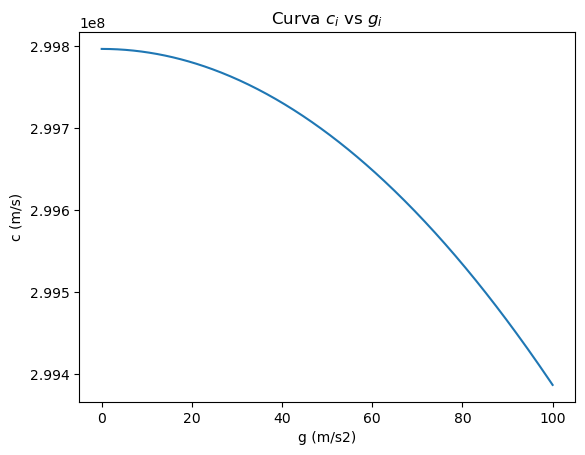
\includegraphics[scale=0.60]{Curva c_i vs g_i.png}
\caption[]{Comportamiento de la ecuación \ref{c_i} como función de $g_i$ en un rango de 0 a 100 m/s$^2$. }
\label{fig:c_itotal}
\end{figure}


\begin{figure}[h]
\begin{center}
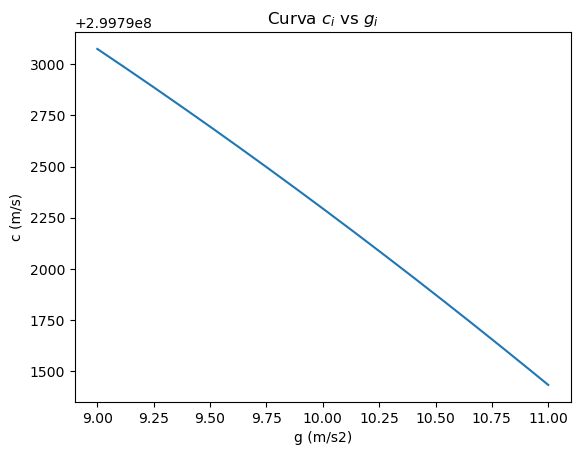
\includegraphics[scale=0.60]{curva c_i vs g_i zoom.png}
\caption[]{Comportamiento de la ecuación \ref{c_i} como función de $g_i$ en un rango de 9 a 11 m/s$^2$. }
\label{fig:c_izoom}
\end{center}
\end{figure}

El resultado de superponer a la línea predicha por la \ac{HCC} los datos proporcionados por Ramdani en la tabla \ref{tab:ramdaniDatos} se tiene en la figura \ref{fig:ramdanisigueHCC}. Se observa que la mayoría de los puntos concuerdan con la predicción dentro de su error, lo cual constituye la última de las justificaciones del presente trabajo.  

\begin{figure}[hbt]
\begin{center}
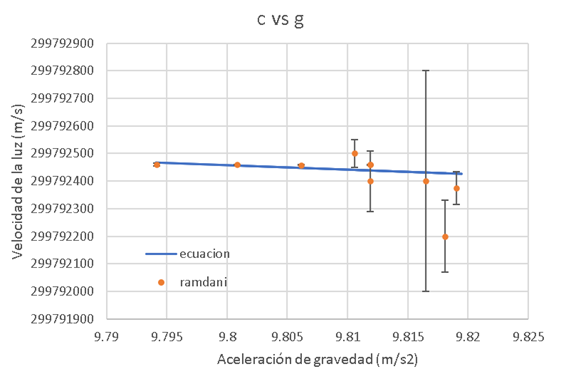
\includegraphics[scale=1]{Imagen4.png}
\caption[]{Datos de velocidad de la luz vs gravedad incluidos en \ref{tab:ramdaniDatos} superpuestos a la linea predicha por \ac{HCC} en la ecuación \ref{c_i}}
\label{fig:ramdanisigueHCC}
\end{center}
\end{figure}


\section{Resultados esperados}

Con el fin de confirmar o refutar la Hipótesis de Céspedes-Curé, se plantea realizar mediciones precisas en tres localidades con diferente valor local de la gravedad, a saber  el campus de la \ac{USB} (Altura 1176 m. Gravedad 977967,685 miligales), en la localidad del teleférico de Caracas (2119 m. 977779,400 miligales) y en la población de Carmen de Urea (Altura  20,36 m. 978251,240 miligales); los valores de la gravedad fueron proporcionados por la Doctora Nuris Orihuela \cite{comunicacionpersonal}. Al aplicar la ecuación \ref{c_i} a cada localidad se tiene que la velocidad de la luz en esos puntos geográficos está dada por los valores incluidos en la tabla \ref{tab:Valores_c_esperados}. Vemos entonces  que los valores de $c$ difieren a partir de la novena cifra significativa, por lo que el mayor reto de la verificación experimental es lograr medidas suficientemente precisas para poder discernir el efecto de la \ac{HCC}.

\begin{table}[h]
\centering
\begin{tabular}{|l|l|l|}
\hline
Localidad & Gravedad m / s² & Velocidad C m / s \\
\hline
Carmen de Urea & 9.7825124 & 29979247\textcolor{blue}{1.69} \\
\hline
USB & 9.77967685 & 29979247\textcolor{blue}{3.97} \\
\hline
Teleférico & 9.777794 & 29979247\textcolor{blue}{5.47} \\
\hline
\end{tabular}
\caption{Valores de gravedad y velocidad de la luz esperada en diferentes localidades, señalando en azul los digitos diferentes entre ellos.}
\label{tab:Valores_c_esperados}
\end{table}


\section{Implicaciones de la HCC}
De demostrarse cierta, la Hipótesis de Céspedes-Curé tendría grandes implicaciones en la física sobre todo en la astronomía, algunas de ellas son:
 \begin{itemize}
     \item \textbf{Explicación a la curva de rotación plana de las galaxias:} Al estudiar como se comporta la velocidad orbital de las estrellas en una galaxia como función de la distancia radial del centro de la misma, se ha encontrado que para una gran parte de los valores más grandes de distancia la velocidad es constante. Para un sistema de este tipo, en el que la mayor cantidad de la masa está en el centro, se espera que la velocidad orbital disminuya con la distancia como pasa, por ejemplo, con los planetas en el sistema solar. Las galaxias tiene mayor masa en su centro, esto se puede saber debido a la gran luminosidad de los mismos debida a la alta densidad de estrellas en esa zona, en comparación con los bordes. Por lo tanto, las velocidades esperadas y las observadas discrepan mucho en su comportamiento, esto ha llevado a interpretar que existe una gran masa distribuida de forma uniforme en las galaxias y la cual no emite luz, la cual se llamó materia oscura. Sin embargo, la \ac{HCC} puede demostrar que la discrepancia de la velocidad se debe, una vez más, a que el efecto Doppler no funciona correctamente por ignorar que la velocidad de la luz es distinta en la región en la que se encuentra la galaxia. De hecho, las estrellas cerca de los bordes experimentan una densidad de energía gravitacional adicional que no perciben las estrellas del centro: la densidad debida a la propia galaxia. Es así como la hipótesis puede solucionar el problema actual de encontrar la materia oscura, simplemente no existe.

\begin{figure}[hbt]
\begin{center}
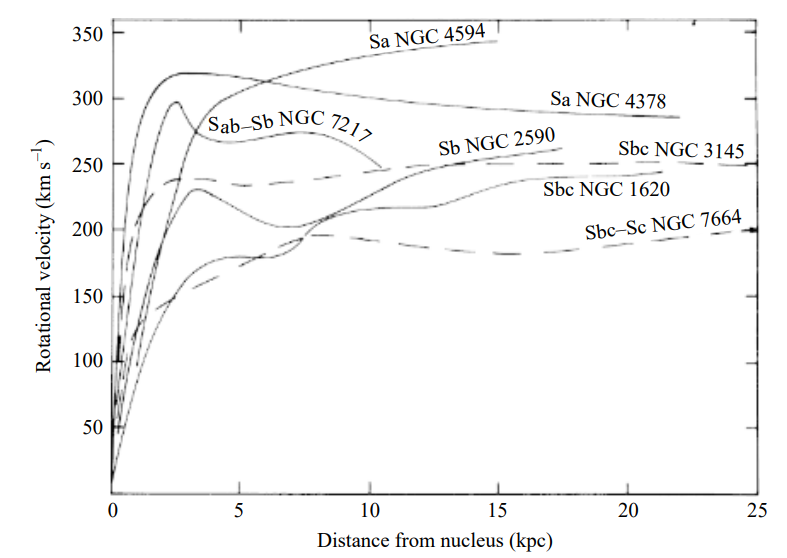
\includegraphics[scale=0.8]{CurvaPlanaGalaxias.png}
\caption[]{Una serie de curvas de rotación para galaxias espirales (figura 24.27 del libro \textit{An introduction to Modern Astrophysics}  \cite{introductiontoastro})}
\label{fig:curvaPlana}
\end{center}
\end{figure}

     \item \textbf{Explicar la expansión acelerada del universo:}  A partir del corrimiento Doppler que muestran las galaxias más lejanas se ha determinado que el universo se expande aceleradamente. Si se asume un universo en expansión con una distribución de masa limitada, la densidad de energía gravitatoria disminuiría hacia los límites, lo que llevaría a un índice de refracción $n'$ cada vez más pequeño y a una velocidad efectiva de la luz $c'$ que aumentaría, resultando en valores sobreestimados de las velocidades de las estrellas deducidas del corrimiento Doppler.

     \item \textbf{Deflexión de la luz de las estrellas por el Sol durante los eclipses solares:} \ac{JCC} en su libro \cite{bib:el-libro} explica este comportamiento de la luz como un fenómeno de refracción causado por el índice de refracción en la vecindad del Sol, que a su vez depende de la densidad de energía gravitacional.

     \item \textbf{Nueva explicación a la existencia de agujeros negros:} Sí se consideran objetos celeste super masivos la densidad de energía gravitacional en su cercanía se hace excesivamente grande, así la \ac{HCC} predice unos valores de velocidad de la luz tan pequeños que percibiríamos el objeto completamente negro \cite{propiedadesdelespaciovacio}.
     
 \end{itemize}

%AL TERMINAR EL CAPITULO PUEDES COMPRAR PAPELERÍA-tres clases del curso de acuarelas


